\section{Introduction}
\label{sec:intro}

\iffalse
\begin{figure}[t]
\centering
	\subfloat[Unordered communication.\label{fig:lightcone-traditional}]
	{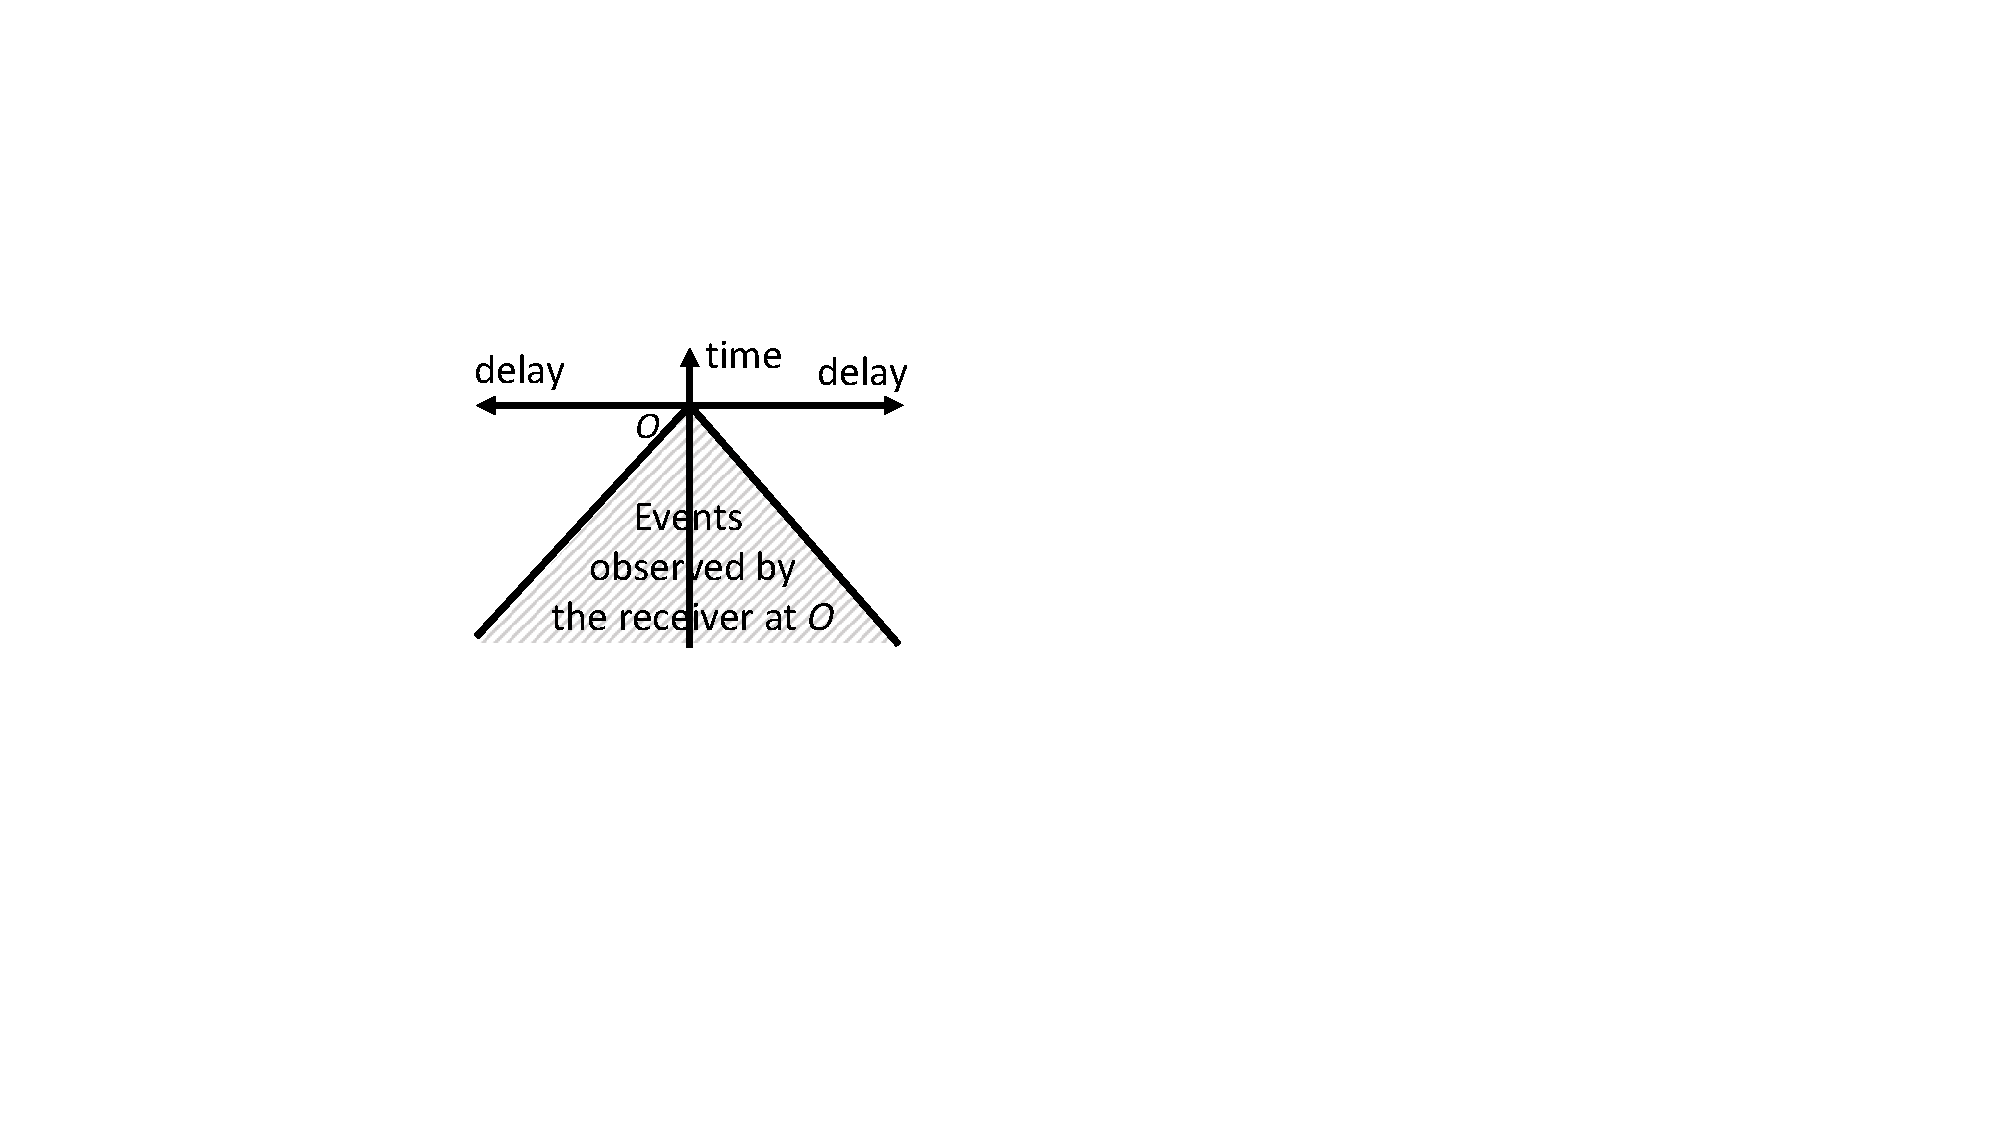
\includegraphics[width=.23\textwidth,page=1]{images/cropped_lightcone.pdf}}
	\subfloat[Total order communication.\label{fig:lightcone-toms}]
	{\includegraphics[width=.23\textwidth,page=2]{images/cropped_lightcone.pdf}}
	\caption{Light cone of observed events by a receiver.}
	\label{fig:lightcone}
    \vspace{-15pt}
\end{figure}
\fi

%Today's data centers host a variety of distributed systems~\textcolor{red}{cite some papers here} to provide service for global users. 
Traditionally, in a network with arbitrary delays, messages are not garanteed to be delivered in a consistent order. For example, multiple shards of a distributed database generate logs to multiple replicas. Each replica may receive logs from shards in a different order. Without special care, such inconsistent ordering may violate data consistency. Solutions that mitigate this problem often introduce synchronization overhead, and often complicate distributed system design.

%\textcolor{red}{describe side effects, e.g., violating data consistence}.
%For example, multiple shards of a distributed database generate logs to multiple replicas, and each replica may receive logs from the shards in a different interleaving ordering.
%The ability to order events in a distributed system is essential for the correctness of many distributed protocols~\cite{lamport1978time,chandy1985distributed}.

%Total order communication provides an abstraction where different receivers process messages from senders in a consistent order. In a total order communication system, messages are tagged with monotonic \textit{event timestamps} by sender, and each receiver processes all messages sent to it based on timestamp order. In log replication, each replica will receive logs in a consistent ordering, which can be an important building block for both strongly consistent and eventually consistent systems. In addition, total order communication can improve consistency in distributed shared memory, as well as accelerate transactional key-value stores~\cite{ports2015designing, eris}, fault-tolerant consensus~\cite{li2016just} and state machine replication~\cite{state-machine-replication}.

Total order communication provides an abstraction where different receivers process messages from senders in a consistent order~\cite{kshemkalyani2011distributed}. More formally, in total order communication, for each pair of processes $P_i$ and $P_j$ and for each pair of messages $M_x$ and $M_y$ that are delivered to both processes, $P_i$ is delivered $M_x$ before $M_y$ if and only if $P_j$ is delivered $M_x$ before $M_y$. 
%In a total order communication system, messages are tagged with monotonic \textit{event timestamps} by the sender. The receiver processes arrival messages based on the timestamp order. In log replication, each replica will process logs in a consistent order, which can be 
Total order communication is an important building block for both strongly consistent and eventually consistent systems. The primitive can improve consistency in distributed shared memory, as well as accelerate transactional key-value stores~\cite{ports2015designing, eris}, fault-tolerant consensus~\cite{li2016just} and state machine replication~\cite{state-machine-replication}.


%Totally ordered message scattering provides an abstraction with a new view of space-time, where different receivers process messages scattered from senders in a consistent order (Figure~\ref{fig:light-cone} (b)). In a total order message scattering system, messages are total order with \textit{event timestamps}, and each receiver receives all messages scattered to it in the timestamp order. This can simplify and accelerate many distributed applications, \textit{e.g.}, transactional key-value stores~\cite{ports2015designing, eris}, total store ordering in distributed shared memory~\cite{}, fault-tolerant consensus~\cite{li2016just}, mutual exclusion~\cite{lamport1978time}, state machine replication~\cite{lamport1978time,lamport1978implementation} and distributed snapshots~\cite{chandy1985distributed}.

%The ordering of events is fundamental to distributed systems.
%The ability to \textit{total order} events in a distributed system, \textit{i.e.}, all nodes observe a consistent ordering of all events, can lead to simple and efficient implementation of a wide range of distributed applications, \textit{e.g.}, transaction processing~\cite{ports2015designing, eris}, transactional key-value stores~\cite{ports2015designing, eris}, fault-tolerant consensus~\cite{li2016just}, mutual exclusion~\cite{lamport1978time}, state machine replication~\cite{lamport1978time,lamport1978implementation} and distributed snapshots~\cite{chandy1985distributed}.
%A total ordering of events indicates that each event can be tagged with a \RED{\textit{logical timestamp}}, and each node observes events in increasing timestamp order (break ties by origin node ID).

%In a networked system, effects of an event propagate via network messages. This means to \textit{scatter} messages from the origin node to a set of receiver nodes. For communication efficiency, an event may not need to be observed by all nodes, and different nodes may receive different messages originated from a same event, so generally it is a \textit{scattering} instead of a \textit{broadcast} or \textit{multicast}. Messages are tagged with the timestamp of the origin event. A node observes an event by receiving the corresponding message. Consequently, from a receiver's perspective, \textit{total ordering of input message timestamps implies total ordering of its observed events}.

Since the dawn of distributed system research~\cite{lamport1978time}, many efforts have been made to achieve total-order broadcast and multicast~\cite{defago2004total}.
%In this paper, we consider a more general form of communication, namely \emph{message scattering}. Message scattering is a common communication pattern where a sender sends (potentially different) messages to multiple receivers. In contrast, identical messages are sent in multicast and broadcast. In a total order message scattering system, different receivers will process scattered messages in a consistent order. Assume $S_1$ scatters $M_1, M'_1$ and $S_2$ scatters $M_2, M'_2$. If $M_1$ is processed before $M_2$ at receiver $A$, then the same processing order should be kept at receiver $B$, \textit{i.e.}, $B$ will process $M'_1$ before $M'_2$.
%Most total order multicast algorithms can be used to implement total order message scattering with some modifications.
However, existing solutions suffer from scalability or efficiency limitations. One line of work leverages logically centralized coordination, \textit{e.g.}, centralized sequencers~\cite{eris}, or tokens to be passed among senders and receivers~\cite{rajagopalan1989token,kim1997total,ekwall2004token}. As a result, it is challenging to scale the system. Another line of work uses fully distributed coordination, \textit{e.g.}, add a consensus round among receivers before they start to process messages~\cite{lamport1978time,chandra1996unreliable}. This causes extra network communication overhead and delay, thus degrading system efficiency.
%An additional limitation comes from the semantics of multicast, where each receiver must get a same sequence of messages. 
More over, an additional restriction comes from the semantics of multicast, where all the receivers must receive identical messages.

In this work, we seek a solution to provide efficient and scalable total-order communication for distributed systems.
First, we generalize multicast to \textit{message scattering}~\cite{}, a more general communication pattern where a sender sends potentially different messages to multiple receivers. Message scattering is a common communication pattern in a distributed system. For instance, in distributed storage, a client writes metadata to a site and data to another site, while other clients read them concurrently. Consistency between metadata and data requires \textit{total-order message scattering} (\sys), which ensures a group of messages to be scattered atomically at the two sites.
%For instance, web servers send an access log and an error log of each HTTP request to different log collectors. Achieving consistent ordering of requests between access and error logs requires \textit{total-order message scattering} (\sys), which ensures a group of messages to be scattered atomically.
%Assume $S_1$ scatters access log $A_1$ and error log $E_1$, while $S_2$ scatters $A_2$ and $E_2$. If $A_1$ is processed before $A_2$ at access log collector, then error log collector should process $E_1$ before $E_2$.
%Logically, a \sys network resembles a FIFO where messages in a same \textit{scattering} are enqueued atomically, and messages are dequeued by receivers in FIFO order.

In this paper, we focus on data center context. Unlike Internet, a data center network (DCN) has a number of desirable properties for distributed systems design, such as regular topologies~\cite{leiserson1985fat,greenberg2009vl2} and single administrative domain. Furthermore, programmable switches start to flourish in data center networks, providing more flexible packet processing. Recently, there has been a trend to co-design distributed systems with underlying data center networks~\cite{eris,netcache-sosp17,dang2016paxos}. Following this trend, we propose \sys to achieve efficient and scalable total order message scattering in a programmable data center network.
 
%Since the dawn of distributed systems research~\cite{lamport1978time}, there has been considerable amount of literature on total-ordering events and input messages using \textit{total order broadcast}~\cite{defago2004total}.
%Most total-order broadcast algorithms can be modified to implement total-order message scattering, but they have scalability or efficiency limitations.
%One line of work uses logically centralized coordination, \textit{e.g.}, using one or more centralized sequencers~\cite{eris}, or have a token to be passed among senders or receivers~\cite{}. The throughput of such systems is hard to scale.
%Another line of work uses fully distributed coordination, \textit{e.g.}, add a consensus round among receivers after they receive the messages~\cite{}. The network communication overhead and additional consensus delay are not negligible.


%Different from the traditional assumption that the network is an unreliable blackbox, a datacenter network has a regular topology and a single administrative domain.
%Recent years, as programmable network switches flourish, there has been a trend to co-design the network with distributed systems~\cite{}. By offloading end-host computation to network switches, key-value stores can be load balanced better~\cite{} and distributed coordination can be simple and fast~\cite{eris}.
%This paper follows this trend and shows that in programmable datacenter networks, total-order message scattering can achieve high performance, be scalable both inside and across data centers, without changing existing network infrastructure.

At its core, \sys separates the bookkeeping of order information from message forwarding. \sys attaches a timestamp to each message at the sender side, forwards them as usual in the network, and buffers them at the receiver side. The switch aggregates timestamp information of all messages to derive the \textit{barrier} for each receiver. The barrier is essentially the \textit{lower bound} of the timestamps of all future arrival packets. With this information, the receiver reorders messages below the barrier and deliver them to applications. \sys is scalable as the switches and end hosts form a decentralized system where control plane communication only takes place between directly connected nodes.

To ensure \sys's efficiency and reliability, we still need to solve three main challenges: 1) How to derive timestamp barriers? 2) How to assign event timestamps? and 3) How to handle packet losses and node failures?

To solve the first challenge, we first generalize timestamp barriers from end hosts to every link in the network. Each switch keeps per-link barrier information and updates it for each packet. If some hosts or links are temporarily idle, we periodically generate beacons carrying barrier information. (Sec.\ref{sec:beacon}). We further merge barriers hierarchically at switches to reduce the amount of beacon traffic (Sec.\ref{sec:ideal}).

For the second challenge, physical clock synchronization seems to be a straightforward solution. However, it does not account for the network latency difference incurred by the OS and links, making fast links constantly waiting for slow links.
%For example, two messages are transmitted from two senders to the same receiver at the same physical time. However, they arrive at different times due to their different network path lengths. As a result, the earlier one must wait for the later one to be processed together.
To minimize the impact, we propose \textit{minimax clock synchronization} (Sec.\ref{sec:sync}) to synchronize logical clocks on each node and assign timestamps to events according to the logical clocks.

For the third challenge, we are aware that data centers are typically well engineered and have very low packet loss rates~\cite{ports2015designing}. We detect packet loss via counters in network switches, and rely on end hosts to retransmit lost packets (Sec.\ref{sec:lossy}). The system is fault tolerant with regard to switch failures. To cope with node failure, \sys achieves atomic delivery using a mechanism similar to two-phase commit (Sec.\ref{sec:failure}).

%In Sec.\ref{sec:lossy}, we add reliability to total-order message scattering in lossy networks, with overhead of one round-trip delay. 


%A simple existing approach to total order messages to the end hosts is called \textit{determin istic merge}~\cite{hadzilacos1994modular, aguilera2000efficient}, which serialize network messages at each network switch. However, commodity switches do not have enough buffer capacity and the programmability to \textit{merge sort} ingress streams (cite PIFO).

%In this work, we propose a different approach to achieve total order scattering. The messages are forwarded as normal in network switches and buffered in end-host receivers. Network switches aggregate timestamp \textit{barrier} information to indicate the \textit{lower bound} of all future timestamps that can be received by an end host. The end hosts reorder messages below the timestamp barrier and deliver them to applications.
%Two challenges arise: \textit{How to derive timestamp barriers? How to assign event timestamps?}

%To derive timestamp barriers, we generalize timestamp barriers from end hosts to every link in the network. A barrier packet on a link indicates the lower bound of the timestamps of all packet that can arrive on the link after the particular barrier packet. To avoid exponential number of barrier packets, barriers are merged hierarchically on network switches (Sec.\ref{sec:ideal}).
%When some hosts or network links are temporarily idle, beacons are sent (Sec.\ref{sec:beacon}).
%Because packet loss in datacenter networks are rare~\cite{ports2015designing}, we could follow the end-to-end principle in system design~\cite{saltzer1984end} and leave packet loss detection and recovery to applications, as in~\cite{ports2015designing,li2016just}.
%In Sec.\ref{sec:lossy}, we add reliability to total-order message scattering in lossy networks, with overhead of one round-trip delay.

%Solving the first challenge ensures correctness of our design. The second challenge, namely assignment of event timestamps, affects efficiency of the design.
%If an event source assigns its messages with very high timestamps, on the receiver end, its messages need to wait in the buffer for a long time for the packets with lower timestamps from other event sources to arrive.
%Our goal is to minimize \textit{reordering delay} from receiving the message to delivering it to the application.
%Physical clock synchronization does not account for the difference in delays incured by OS network stacks and network links.
%In Sec.\ref{sec:sync}, we propose \textit{minimax clock synchronization} to synchronize logical clocks on each node and assign timestamps to events according to the logical clocks, so that messages originated from distant nodes with adjacent timestamps arrive at receivers as simultaneously as possible.

For evaluation, We implement three incarnations of \sys on network devices with different programming capabilities. Sec.\ref{sec:p4} introduces the implementation on state-of-the-art reconfigurable switches~\cite{tofino,cavium} that supports flexible stateful per-packet processing. Sec.\ref{sec:commodity} presents the implementation on fixed-function switches with a CPU~\cite{arista}, which can process control packets but not every data packets. In case switch CPUs do not have enough processing capacity, Sec.\ref{sec:end-host} uses end hosts for control plane processing.

%Sec.\ref{sec:p4} assumes stateful per-packet processing with data-plane programmable switches. Sec.\ref{sec:commodity} assumes commodity switches with a programmable CPU, which can process control packets but not each and every data packets. In case switch CPUs do not have enough processing capacity, Sec.\ref{sec:end-host} uses end hosts for control plane processing.

%We design and implement \sys with different programming capabilities of network switches. Sec.\ref{sec:p4} assumes stateful per-packet processing with data-plane programmable switches. Sec.\ref{sec:commodity} assumes commodity switches with a programmable CPU, which can process control packets but not each and every data packets. In case switch CPUs do not have enough processing capacity, Sec.\ref{sec:end-host} uses end hosts for control plane processing.

\textcolor{red}{We evaluate the performance of \sys using both small-scale testbed experiments and large-scale xxxx.}

\sys achieves low reordering delay and low network overhead and CPU processing overhead in both small and large system scales. \sys is also fault tolerant and supports incremental deployment, as new hosts, switches and links can join the system within only one RTT. As a case study, Sec.\ref{sec:application} shows that \sys achieves 6.4 million transactions per server and 40~$\mu$s latency for one-shot transactions in YCSB+T~\cite{dey2014ycsbt} transactional key-value store, which is 10x efficient than other systems and close to the performance of a non-transactional system. For New-Order and Payment transactions in TPC-C~\cite{tpcc} benchmark with 4 districts, \sys scales to thousands of concurrent clients, while other concurrency control mechanisms only scale to tens of clients. \sys can also achieve scalable serializable log replication.

\textcolor{red}{Do we need to add: the rest of the paper is orgainized as follows. .....}
